% !TEX root = Eco-Model.tex
\section{Problem Background} % (fold)
\label{sec:problem_background}

\subsection{Cloud Manufacturing Ecosystem} % (fold)
\label{sub:cloud_manufacturing_ecosystem}
As an application of Networked Manufacturing, Cloud Manufacturing proposed by ...

(problems background to form the ecosystem)

Combined with the problem background and other scholars' previous work, we proposed an improved framework that suits for Cloud Manufacturing environment as shown in \autoref{fig:structure}.
\begin{figure}[htbp]
\centering
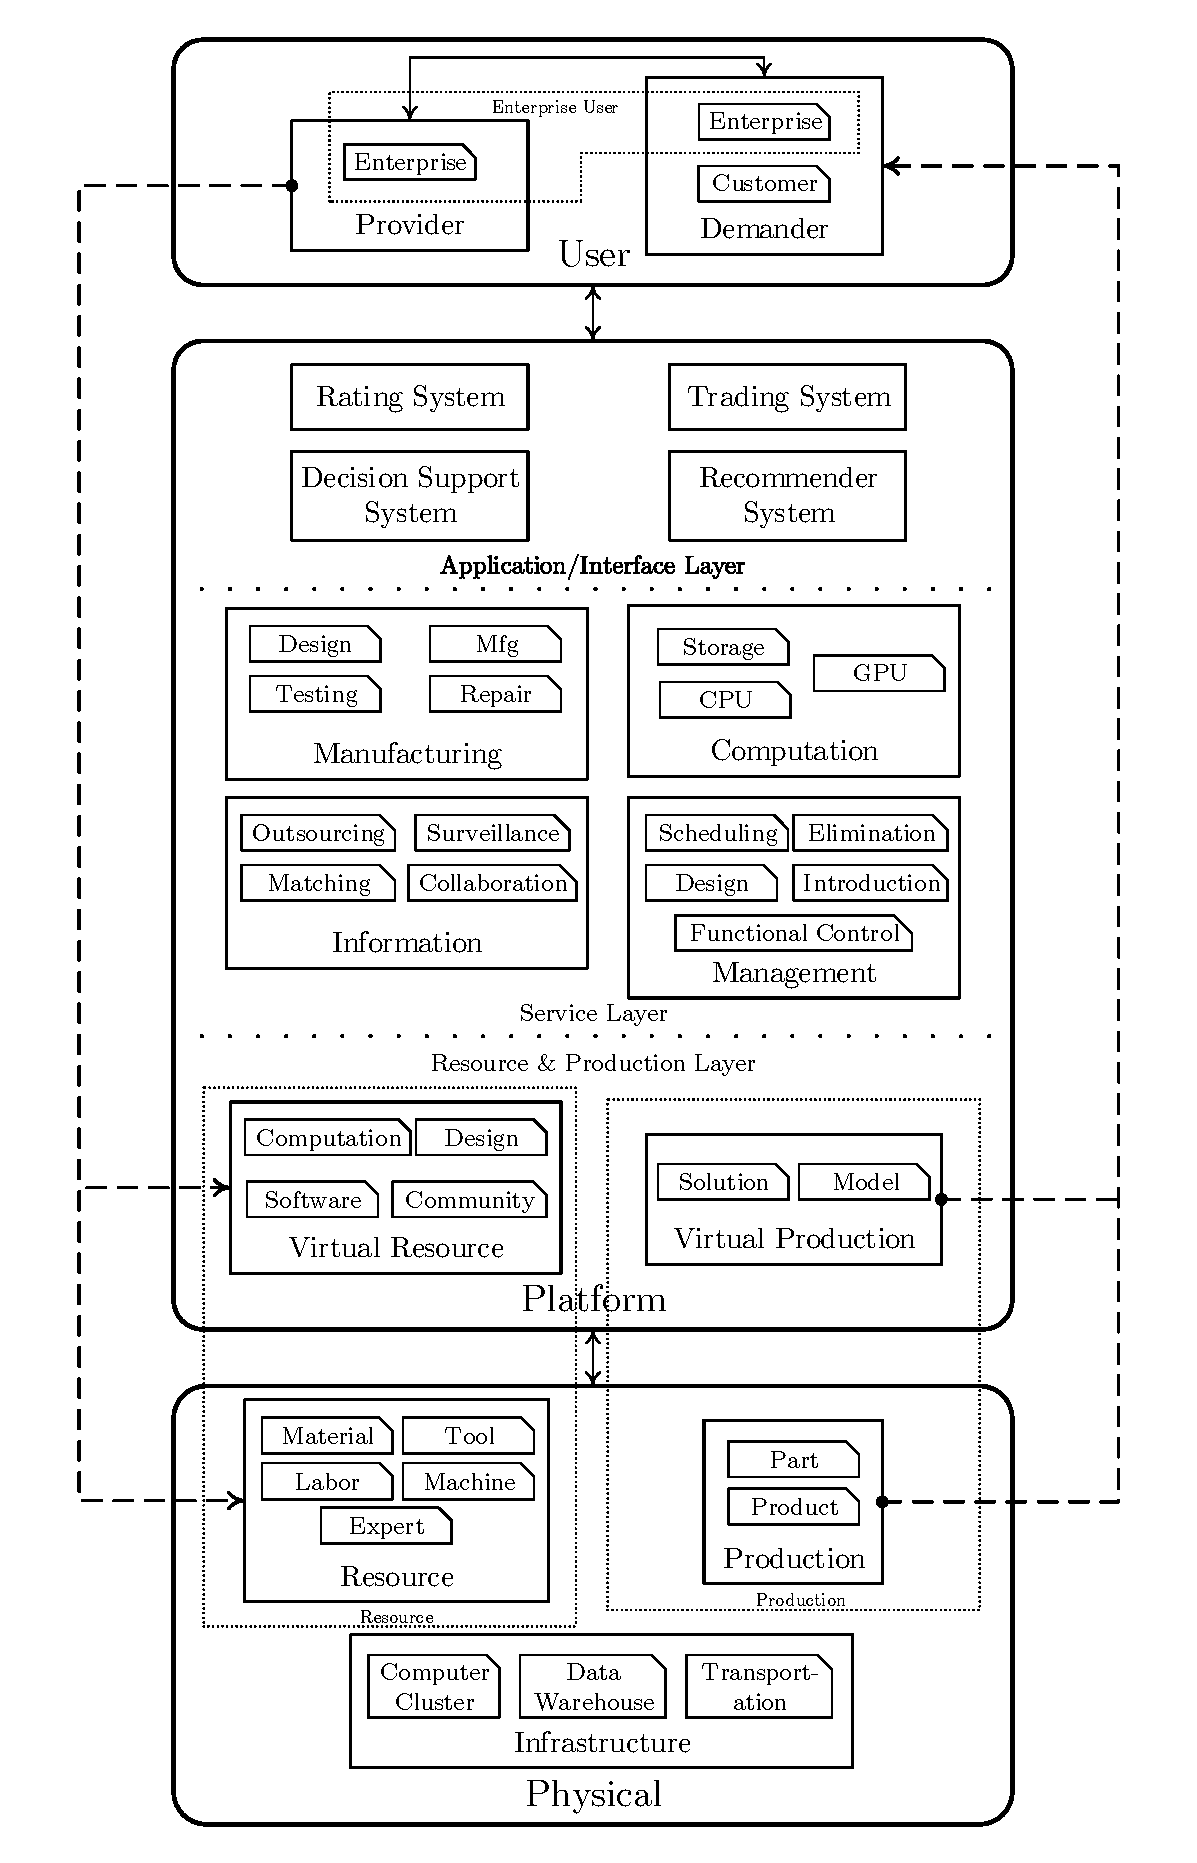
\includegraphics[scale = .6, trim = 0 15 0 35]{Cloud_Mfg_Structure.pdf}
\caption{Cloud Manufacturing Architecture with Main Flows}
\label{fig:structure}
\end{figure}

\begin{figure}[htbp]
\centering
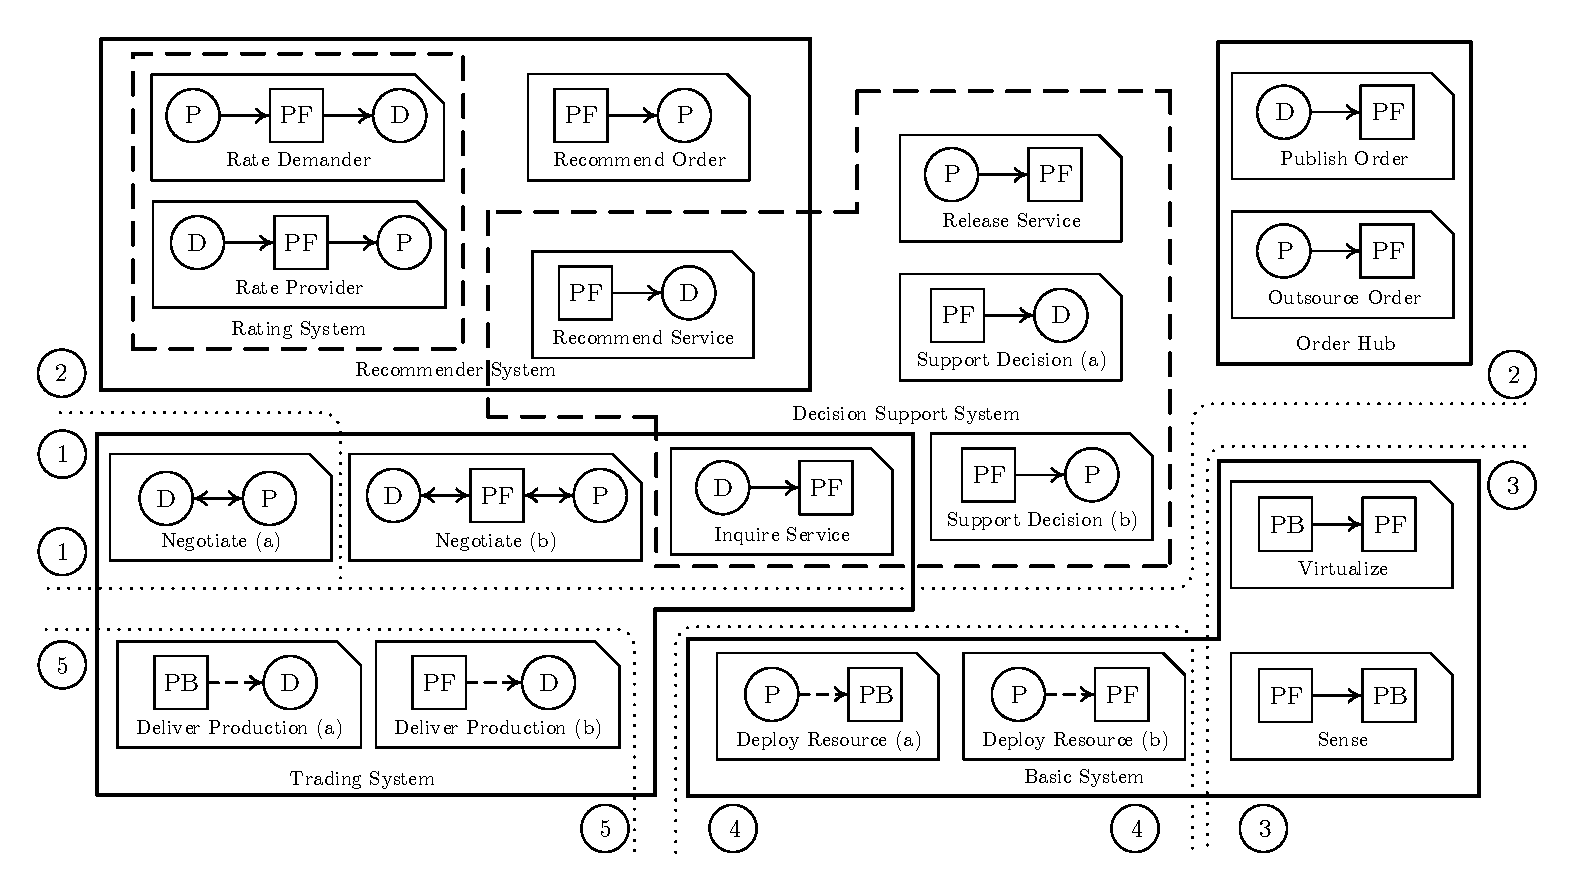
\includegraphics[scale = .6, trim = 0 15 0 10]{supplementary.pdf}
\caption{Supplementay Illustration of \autoref{fig:structure}}
\label{fig:supplementary}
\end{figure}

The architecture of Cloud Manufacturing is mainly comprised by three parts, namely, \begin{inparaenum}[1)]
\item User,
\item Platform and
\item Physical Base
\end{inparaenum}, some of whose subparts are connected by material or information flows. With the supplementary illustration of \autoref{fig:supplementary}, which categorizes the main applications in Cloud Manufacturing environment with the forementioned flows that marked by circled number (i.e. \textcircled{\small{1}}), a simple version of conception for Cloud Manufacturing architecture we study here can be described as follows:


Modular approaches are widely used to decompose a complex system into smaller subsystems according to their functions. For example, Yang and Li (2011) divided a cloud manufacturing services management and control platform into seven functional modules such as system management module, production management module and so on

\subsubsection{Enterprise Business Mode}

\subsubsection{Resource Sharing Mechanism}

\subsubsection{Ecosystem Adjustment}

% subsection cloud_manufacturing_ecosystem (end)

\subsection{Main Copmlexity Concepts} % (fold)
\label{sub:main_copmlexity_concepts}

\subsubsection{Self-organization}

\subsubsection{Emergence}

\subsubsection{Co-evolution}

\subsubsection{Adaption}
% subsection main_copmlexity_concepts (end)

\subsection{Ecosystem Evolvement} % (fold)
\label{sub:ecosystem_evolvement}

% subsection ecosystem_evolvement (end)

\subsection{Optimal Guidance} % (fold)
\label{sub:optimal_guidance}

% subsection optimal_guidance (end)
% section problem_background (end)